\documentclass[12pt,a4paper]{article}
\usepackage[UTF8]{ctex}
\usepackage{amsmath,amssymb}
\usepackage{listings}
\usepackage{xcolor}
\usepackage{hyperref}
\usepackage{geometry}
\usepackage{graphicx}
\geometry{margin=2.5cm}

\lstdefinestyle{python}{
  language=Python,
  basicstyle=\ttfamily\small,
  keywordstyle=\color{blue}\bfseries,
  commentstyle=\color{gray},
  stringstyle=\color{red},
  showstringspaces=false,
  breaklines=true,
  frame=single,
  backgroundcolor=\color{gray!10}
}

\title{Shor's Algorithm / Shor 算法}
\author{QuoNic}
\date{}

\begin{document}
\maketitle

\begin{center}
\textbf{Algorithms / 算法} | 难度：高级 | 预计时间：25 分钟
\end{center}

\tableofcontents
\newpage

\section{为什么需要？}

Shor 算法可以在多项式时间内分解大整数，威胁 RSA 加密体系。

\subsection{经典局限}
\begin{itemize}
  \item 经典算法（如数域筛法）需要亚指数时间
  \item RSA-2048 经典分解需要数千年
  \item 经典算法无法有效利用量子并行性
\end{itemize}

\subsection{量子优势}
\begin{itemize}
  \item Shor 算法需要 $O((\log N)^3)$ 时间
  \item RSA-2048 量子分解只需数小时
  \item 是量子计算最著名的应用之一
\end{itemize}

\subsection{实际应用}
\begin{itemize}
  \item 密码学（破解 RSA）
  \item 后量子密码学（推动新标准）
  \item 数论（分解大整数）
\end{itemize}

\section{快速上手}

\begin{lstlisting}[style=python]
from quonic.algorithms import shor

# Factor N = 15
result = shor(15)
print(f"Factors: {result.factors}")
\end{lstlisting}

\textbf{预期输出}：
\begin{verbatim}
Factors: [3, 5]
\end{verbatim}

\section{原理详解}

\subsection{电路图}

\begin{center}
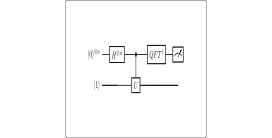
\includegraphics[width=0.7\textwidth]{../../images/shor_circuit.svg}
\end{center}

\subsection{数学推导}

Shor 算法的核心是寻找周期 $r$：
\begin{equation}
a^r \equiv 1 \pmod{N}
\end{equation}

\textbf{算法步骤}：
\begin{enumerate}
  \item 选择随机 $a < N$
  \item 用量子计算寻找 $a^x \mod N$ 的周期 $r$
  \item 如果 $r$ 是偶数且 $a^{r/2} \not\equiv -1 \pmod{N}$，则 $\gcd(a^{r/2} \pm 1, N)$ 是 $N$ 的因子
\end{enumerate}

\subsection{几何解释}

Shor 算法利用量子傅里叶变换（QFT）提取周期信息。量子计算机同时计算所有 $a^x \mod N$，然后 QFT 提取周期。

\section{代码详解}

\begin{lstlisting}[style=python]
from quonic.algorithms import shor

# shor(N)
# N: integer to factor
result = shor(15)

# result.factors: list of factors
# result.period: period found by QFT
print(f"Factors: {result.factors}")
\end{lstlisting}

\section{进阶用法}

\subsection{场景 1：不同整数}

\begin{lstlisting}[style=python]
# Factor different integers
result_21 = shor(21)   # [3, 7]
result_35 = shor(35)   # [5, 7]
result_77 = shor(77)   # [7, 11]
\end{lstlisting}

\subsection{场景 2：大整数}

\begin{lstlisting}[style=python]
# Larger integers (requires more qubits)
result = shor(2047)  # [23, 89]
\end{lstlisting}

\section{适用场景}

\subsection{密码学}

Shor 算法威胁 RSA 加密，推动后量子密码学发展。

\subsection{数论}

Shor 算法可以高效分解大整数。

\subsection{后量子密码学}

Shor 算法推动了新的加密标准（如 CRYSTALS-Kyber）。

\section{常见问题}

\subsection{Shor 算法能分解多大的数？}

理论上可以分解任意大的数，但需要足够多的量子比特。目前实验上分解了 15、21 等小整数。

\subsection{Shor 算法需要多少量子比特？}

分解 $N$ 需要约 $2\log_2 N$ 个量子比特。分解 RSA-2048 需要约 4000 个逻辑量子比特。

\subsection{Shor 算法会破解所有加密吗？}

Shor 算法只威胁基于大整数分解和离散对数的加密（如 RSA、ECC）。基于格的加密（如 CRYSTALS-Kyber）是安全的。

\section{学习路径}

\subsection{前置知识}
\begin{itemize}
  \item 量子傅里叶变换（QFT）
  \item 量子相位估计（QPE）
  \item 数论基础
\end{itemize}

\subsection{继续学习}
\begin{itemize}
  \item 后量子密码学
  \item 量子纠错
  \item 量子网络
\end{itemize}

\section{完整示例代码}

\subsection{示例 1：基本 Shor 算法}

\begin{lstlisting}[style=python]
from quonic.algorithms import shor

result = shor(15)
print(f"Factors: {result.factors}")
\end{lstlisting}


\section{下载}

\begin{itemize}
  \item [shor.py](https://github.com/ChrisLee0721/QuoNic/blob/main/examples/shor/shor.py)
\end{itemize}

\end{document}
